\documentclass{article}
\usepackage{cite}
\usepackage{graphicx,fancyhdr,amsmath,amssymb,amsthm,subfig,url,hyperref}
\usepackage[margin=1in]{geometry}
\usepackage{comment}
\usepackage{framed} 
\usepackage{indentfirst}
\usepackage{appendix}
\usepackage{bbm}
\usepackage{algorithmic}
\usepackage[ruled,vlined]{algorithm2e}
%%Algorithm2e documentation
% http://tug.ctan.org/macros/latex/contrib/algorithm2e/doc/algorithm2e.pdf
%\usepackage{algorithm}
\usepackage{courier}

%%%%%%
\SetKwProg{Fn}{Function}{}{}
%%%%%%
%----------------------- Macros and Definitions --------------------------

%%% FILL THIS OUT
\newcommand{\projectname}{Algorithmic Preference Matching in the Department of Defense}
%%% END

%\renewcommand{\theenumi}{\bf \Alph{enumi}}

%\theoremstyle{plain}
%\newtheorem{theorem}{Theorem}
%\newtheorem{lemma}[theorem]{Lemma}

\fancypagestyle{plain}{}
\pagestyle{fancy}
\fancyhf{}
\fancyhead[LO,RE]{\sffamily\bfseries\large \projectname}
% \fancyfoot[LO,RE]{\sffamily\bfseries\large ianedwardshaw (at) gmail.com}
\fancyfoot[RO,LE]{\sffamily\bfseries\thepage}
\renewcommand{\headrulewidth}{1pt}
\renewcommand{\footrulewidth}{1pt}

\graphicspath{{figures/}}

%-------------------------------- Title ----------------------------------

\title{\projectname}
\author{Ian Shaw \thanks{Ian Shaw (Lieutenant JG, US Navy) is a cyber warfare engineer. As an alum of Stanford University, he researched sequential machine learning models at the Institute for Computational and Mathematical Engineering. He, and all authors of this piece, graduated with distinction from the US Naval Academy and together make up Naval Algorithms, the small prototype team described in the paper. } 
\and Zac Dannelly \thanks{Zac Dannelly (Lieutenant JG, US Navy) is a cryptologic warfare officer serving at Fort Meade. He has researched the effects of emerging technologies on organizations through degrees from the Judge Business School at the University of Cambridge, on the Gates Scholarship, as well as from the Management Science and Engineering Department at Stanford University.}
\and Drew Calcagno \thanks{Drew Calcagno (Lieutenant JG, US Navy) serves various teams in the Office of the Secretary of Defense. He writes emerging technology strategy there, particularly regarding artificial intelligence. He is an alum of the University of Oxford as a Rotary Scholar and the University of London as a Fulbright Scholar where he constructed theses on how the Department of Defense and the Intelligence Community could better coordinate counter-terrorism operations, particularly on the African continent.} 
\and Richard Kuzma \thanks{Richard Kuzma (Lieutenant JG, US Navy) is a Navy surface warfare officer passionate about how the Defense Department adapts to emerging technologies, particularly artificial intelligence. He is an alum of the Harvard Kennedy School where he wrote a thesis on how the Defense Department should structurally change to implement artificial intelligence, partnering with the Defense Innovation Unit. He is an associate at Harvard’s Technology and Public Purpose Project. He is on Twitter, @rskuzma.}} 

%--------------------------------- Text ----------------------------------

\begin{document}
\maketitle

\begin{abstract}
The Department of Defense maintains a consistent matching problem in the placement of military members into jobs due to the requirement that uniformed service members rotate positions every three years. Gale and Shapely provided a stable matching process 1962 \cite{1962_Gale} that if applied to this problem would greatly improve the current, manual matching process. In this paper we go a step further noting that mixed-integer programming can be applied in the matching process to sacrifice stability in favor of military leadership goals. Additionally, we glean novel metrics from the expressed ordered preferences of both service members for jobs as well as job owners’ preferences for service members. These metrics are: specialization, competitiveness, similarity, and preference correlation. We formulated our prototype for the Chief of Naval Personnel. Nevertheless, our work is agnostic and can be applied not only to any service branch, but to any matching market not requiring stability, defined by obliged market participants.  \footnote{The code to demonstrate the matching algorithms, optimization, and preference-based metrics can be found in Ian Shaw's \texttt{Dynamic\_Manning} Github Repository . \url{https://github.com/ieshaw/Dynamic_Manning}}

\end{abstract}

\newpage

\tableofcontents

\newpage

\section{Introduction}

Under the backdrop of the President of the United States issuing the \textit{Executive Order on Maintaining American Leadership in Artificial Intelligence} in February 2019, we created the algorithmic foundation for the advancement of artificial intelligence and machine learning (AI/ML) in military talent allocation.  Before the US Government can accomplish its AI/ML goals, however, it must embrace the essential building blocks underlying the buzzwords. 

We believe the world to be arcing toward the need for humans to grow as increasingly specialized workers, and in the vicious games of statecraft and warfare, allocating talent with hyper specificity will become a necessity for victory. A building block on that path is the institutional acceptance of data-driven human decision making and algorithmic support of those human decisions. To that end, we theorized, coded, and prototyped an mixed integer programming (MIP) algorithm that matches job seekers (sailors) and job owners (commanding officers) more optimally than can any existing Department of Defense (DoD) process, algorithmic or human. 

The process of talent management through ‘detailing’ in the Navy is an arena ripe for such an MIP approach. Due to the structure of many sailors applying to jobs  with possibly more than one opening, this issue is a rendition of the college admission problem \cite{1962_Gale} without the need for stability \cite{1988_Roth_Sotomayor}. The essence of our solution is completed via algorithmic linear programing, specifically the use of MIP. We explore the nuances of how algorithms greatly increase optimal outcomes. Moreover, we discuss how MIP pushes optimality beyond deferred acceptance algorithms which, until now, were considered state-of-the-art for the DoD. 


\section{Problem Description}

Human talent allocation is a resource-intensive process for an institution. This paper outlines the mathematics necessary to lay the groundwork for such a task within one of the most complex institutions of American society -- the DoD.  We dove into this problem seeking to show the validity of the mathematics, as well as to discover the challenges that exist when creating a talent marketplace from the ground up. Furthermore, despite the small prototype sample, the find the algorithm to be widely scalable, particularly if combined with a proper front-end as our project is the back-end of a future full-stack system. 

Market forces are largely the drivers behind a job marketplace -- this concept is not new for the American economy.  However, given a captive audience such as service members ordered to specific jobs, the mathematical benefit of a ‘benevolent autocracy’ is immense.  Rather than the suboptimal fate to which current servicemembers are subjected, the DoD is already shopping for a better way forward algorithmically.  We improve upon what currently exists in all metrics except current implementation; nevertheless, we have a plan with stakeholders to quickly field the technology. 

In the Navy, terminology of a ‘detailing marketplace’ refers to the attempts to ‘detail,’ or place, warfighters into their next job.  This detailing marketplace is a system by which military members can transparently rank their job preferences and the people who ‘own’ those jobs can supply their preference of incoming personnel. This problem is rather unique to the military due to the aforementioned captive market of many members obligated to remain in service due to contract, desiring to stay in for a pension, or perhaps wishing to stay due to a sense of public service. This market type is complemented by an inability for lateral entry -- almost all members need to start from the entry level.  Additionally, servicemembers typically change jobs every one to three years. 

There are ontological parallels to other communities, too. This process is shared in some regards by the medical school graduates applying to the residency stage of their training. Those graduates apply to a pool of US residency programs. This pool is also rather narrow, mostly coming from US based medical schools, and the specificity of skill set required for success is better understood and measured than success as a military officer. 

This general similarity between markets is the reason our initial matching algorithm (Gale-Shapley deferred acceptance algorithm) resembled that of the National Residency Match Program. For context, the Gale-Shapley algorithm's application to the residency matching problem earned the 2012 Nobel Prize in Economic Sciences.

This paper also proposes an optimization-based solution to the matching process. The optimization is not found in the National Residency Match Program due to the need for ‘stability.’ Stability here is exemplified by medical students’ ability to reject their assigned position, a choice rarely given to military members, if at all. Thus, optimization in the military context does not require stability.  As a result, mathematical optimization, unburdened \cite{1984_Roth} \cite{1985_Roth_b} \cite{1989_Roth} by the luxury of stability, is at its peak in our formulation -- a notable improvement. 
We found that a traditional algorithm, like Gale-Shapley deferred acceptance, was unconducive to the creation of modular constraints.  A constraint may be the introduction of a rule based on Navy policy that the algorithm would have to satisfy before conducting all matches (e.g. at least 95\% of  dual-military couples ought to be stationed within 50 miles of their partner). For that reason, we transitioned to mixed integer programming, a more agile linear programming approach to the problem.  We later show that MIP outperforms the deferred acceptance iteration outright, in addition to its ease of introducing constraints without massive re-coding. 

Acknowledging the difficulty of wrangling disparate and dated personnel data, this paper also explores helpful metrics that can be gleaned simply from submitted, ordered preferences by job seekers and job owners. These are specialization, competitiveness, similarity, and preference correlation. These metrics can be used to describe both sides of the market, on the seeker or the owner alike. 
 
Further, the paper ends with suggested metrics that would be gleaned if personnel data beyond mere preferences were accessible, clean, and structured. These include a similarity measure based on quality encodings and a suggested ordering of possible jobs or applicants. AI/ML, specifically deep learning, could enable the latter. The suggested ordering would not make decisions on placement, but rather provide job seekers and job owners with an intelligent ordering, allowing a human participant to more easily distill the vast amount of job information relevant to her. 



\subsection{Solution Description}

Our solution to the talent allocation problem is to optimize the matching of preferences from both sides: job owners (commanding officers) and job seekers (sailors). This general similarity between the military and medical  markets is the reason our investigation builds off the Gale-Shapley deferred acceptance algorithm used in the National Residency Match Program. 

This paper proposes an optimization-based solution to the matching process. The optimization is not found in the National Residency Match Program due to the need for stability. Stability here is defined as a system where no two individuals from opposite sides of a market (male and female in the stable marriage problem) can leave their assigned partners and be better off for it. Stability is necessary for  medical students who have the ability to reject their assigned position, a choice not available to most military members. Thus preference matching in the military context does not require stability. Unburdened by the constraint of stability, we can leverage mathematical optimization \citep{1984_Roth} \citep{1985_Roth_b} \citep{1989_Roth}; this insight is the key to the rest of our investigation. 

We found that a traditional algorithm, like Gale-Shapley deferred acceptance, was unconducive to the creation of modular constraints that common in US Navy personnel policy. One such constraint is the Chief of Naval Personnel's goal to have at least 95\% of dual-military couples stationed within 50 miles of their partner. To gain modularity we turn to binary-integer programming.  We later show that this approach can outperform the deferred acceptance iteration in our desired metrics, in addition to its ease of introducing constraints without massive re-coding. 


\subsection{Algorithm}

The constraints we apply are the same as the college admissions problem \citep{1985_Roth}. The line numbers refer to their mathematical formulation in the binary-integer program of Section \ref{matching}.
\begin{enumerate}
\item Each sailor can only be assigned to one position (\ref{one_job})
\item Either all the jobs are filled or every job seeker is placed (\ref{all_filled})
\item Each job can fill up to but not exceed the allocated number of positions (\ref{capacity})
\end{enumerate}

For the sake of the prototype improving upon deferred acceptance in our desired metrics (explained in Section \ref{windows}) we also include the constraints in line (\ref{s_da}, \ref{o_da}). This constellation of constraints has the added benefit of guaranteed feasibility since the deferred acceptance output is a feasible solution.

Though a comparison to deferred acceptance is of academic interest, we also provide alternate formulations that may be of more pragmatic interest to military leaders. These include co-location (Section \ref{CoLocation}), quality spread (Section \ref{QualitySpread}), weighting the importance of certain command's preferences over others (Section \ref{Importance}), and retention (Section \ref{Retention}).


\subsection{Strategy Proofness}

An important note is the attempt at strategy proofness of the algorithm \citep{2011_Budish} \citep{2006_Atila}, thus creating an incentive for honesty \citep{1982_Roth}. Proper market construction ensures that there is no benefit for a participant to provide incomplete preferences.  Likewise, we must acknowledge that there can be difficulty associated with a market participant ranking an incredibly large number of opportunities. To meet this need, we complete any incompletely provided preferences using the `implied preference’ method\citep{2019_Shaw}. 

The complete strategy proofness investigation of this formulation is left as an aspect of future work, but we acknowledge that there could be benefits to coalitions or awareness of the preference landscape of competitors. There is also a possibility of rejecting the implied preferences, as one market maker concluded unexpressed preferences indicate indifference \citep{1994_Irving} -- an expression of preference all its own. Nevertheless, the strategy proofness of Irving’s approach in an MIP matching process has yet to be explored. In this same vein, the aformentioned 'implied preference' method has not been expanded to to encompass the `separation' preference described in Section \ref{Retention}. 


\section{Metrics}

\subsection{Pre-Match Metrics}

\subsubsection{Competitiveness}

\subsection{Competitiveness}

\subsubsection{Average Ranking}

The competitiveness score for any given job could be defined as the average preference ranking of the job across all seekers.

Consider a set of preferences $\{P^{S}_{y,z} \in \mathbb{Z}^+: y \in \{1, \dots, n\}, z \in \{1, \dots, m\}\}$. This indicates the positive integer preference ranking of the job seeker for the $n$ available jobs and $m$ seekers. 

Thus the competitiveness score $C$ for a given job $j$ could be defined as 

\[\texttt{Competitiveness}_j = \frac{1}{n} \sum_{i=1}^m P^S_{i,j}\]

\subsubsection{Adapted Sciorintino Ratio}

An average of preference rankings, though conveying the desirability of a position, loses mcuh of the information contained in the distribution of preferences. For example, a position ranked first by ten individuals and hundredth by a twenty individuals has the same average ranking as a job ranked seventh by all thirty individuals; yet the prior is much more competitive. 

The Sciorintino Ratio is a metric from the finance industry used to measure the performance of a investment vehicle based on the distribution of their returns. An investment vehicle with consistent, small positive returns is much different than one with consistent negative returns and one big win, even though the average return may be the same. We see the same problem in finance as the detailing marketplace, conveying the nature of a distribution in a single metric. The difference in this ratio as compared to the more popular Sharpe Ratio, is that the Sciorintino ratio does not let positive volatility negatively effect the score, only volatility on the negative side is punishing. Here we want to adapt the the concept that the volatility of preference is reflected only with higher ranked preferences. For example, if a job has an average ranking of ten, the fact that many people ranked it second is much more important for competitiveness than the fact that many other people ranked it thirtieth.

The formulation for our Adapted Sciorintino Ratio for the competitiveness of job $j$ takes the form

\begin{align}
\mu_j &= \frac{1}{n} \sum_{i=1}^m P^S_{i,j} \\
\sigma_j &= \frac{1}{m^2} \mathbbm{1}\big( P^S_{i,j} < \mu \big) \big(P^S_{i,j} - \mu \big)^2
\texttt{Competitiveness}_j &= \frac{\mu_j}{\sigma_j}
\end{align}

\subsection{Specialization}

\[\textit{Definition}\] 
Specialization measures the extent to which the maximum desire for a sailor or job differs from the mean. Sailor A is highly specialized if one job owner highly desires them much more than the mean job owner (e.g. Sailor A is the 1st preference choice of Job Owner X, but is on average the 21st ranked preference). A sailor is a specialist to the extent that their skill set will serve a specific function well, with a comparative advantage to their peers and with a disproportionate positive contribution to the Department of Defense compared to the other roles they are qualified for.

\[\texttt{Specialization}^S_i = \frac{\mu(P^O_i) - \max\{P^O_i\}}{\mu(P^O_i) + \max\{P^O_i\}}\]

\[\textit{Impact}\] 
A sailor with a high specialization has some skill set that will serve a specific job function well; the seeker has an advantage over peers for a single role compared to the other roles the seeker is qualified for. If most job owners rate a seeker with low preference but a single owner rates that seeker with a high preference, the marginal gains of that seeker being matched with that owner are high. Matching the sailor with this particular role utilizes their specialization and produces a disproportionate positive contribution to the Department of the Navy. Intuitively, the matching algorithm will favor creating high-specialization matches. Failing to make these matches has a more negative impact on the system than failing to make non-specialized matches, because the usefulness of the sailor goes down significantly between their optimal match and average matches. This metric may be useful in the future to examine if very particular aspects of jobs or sailors make them attractive to small subsets of the other population.

%\subsection{Preference Correlation}

%Preference correlation is a metric built to understand the alignment of job owner preferences and job seeker preferences. This is the correlation ($R^2$) of a given job owner's preferences and the preferences of seekers for that job. 

\subsection{Post-Match Metrics}\label{post-match}

Preference Allocation Windows
Preference allocation indicates how many individuals received their top preference, how many individuals got a top three, top five, and top 10 preference, and how many failed to be matched with any preference.

Talent Distribution
Some job owners have multiple jobs. Ideally, such job owners would get an approximately equal set of preferences; one owner with five job slots would not get their 1st-5th choices while another job owner with five job slots gets their 20th-25th preferences. 

Preference Difference Gap
This metric helps to illuminate the separation between job owner and sailor preferences. This can be an indicator for senior leaders that neither sailors nor job owners had their preferences unduly weighted within the optimization system.  


\section{Running the Prototype}

\subsection{Overview}

In this report we outline the mathematical basis for a detailing marketplace. We recognize that previous efforts have been attempted in this arena, many failing due to the inaccessibility of Navy personnel data. For this reason, most of this report focuses on what can be accomplished without personnel data, just the submitted preferences of job seekers and job owners.  Sections \ref{Matching} and \ref{Metrics} focus on efforts that would be enabled by only preferences, not until Section \ref{Beyond} do we allude to efforts that could be pursued if further data were available.

\subsection{Notation}

Throughout the paper, we will reference the notation listed in this section.

\begin{align}
m &= \text{number of different jobs available}\\
n &= \text{number of persons}\\
O_i &= \text{set of seekers hired by owner of job $i$} \\
S_i &= \text{job of seeker $i$} \\
E &= \text{Seeker Entity Matrix}, \in \mathbb{Z}^{+, n_e \times 2}\\
e_{i,2} &= \begin{cases}
r & \text{ Seeker $e_{i,1}$ requests co-location with Seeker $r$} \\
0 & \text{ Seeker $e_{i,1}$ does not request co-location}
\end{cases} \\
n_c &= \text{number of couples requesting co-location}\\
&= \sum_{i=1}^n\mathbbm{1}(e_{i,2} == 0) \\
n_e &= n - n_c \\
\vec{P^S_i} &= \text{Preference vector of job seeker $i$, } \in \mathbb{Z}^{+, m \times 1} \\
P^S &= [\vec{P^S_i} | \dots | \vec{P^S_n}] \in \mathbb{Z}^{+, m \times n}, \\ 
&\text{\indent Preference Matrix of Seekers} \\
\vec{P^O_i} &= \text{Preference vector of job owner $j$, } \in \mathbb{Z}^{+, n \times 1} \\
P^O &= [\vec{P^O_i} | \dots | \vec{P^O_n}] \in \mathbb{Z}^{+, n \times m}, \\ 
&\text{\indent Preference Matrix of Job Owners} \\
\vec{A} &= \text{Position Available vector }\in \mathbb{Z}^{+, m \times 1} \\
a_j &= \text{Amount of positions for job $j$, } \in \mathbb{Z}^{+} \\
X &= \text{Placement Matrix} \in \{0,1\}^{n \times m} \\
x_{i,j} &= \begin{cases}
1 & \text{if $S_i$ is slated for job $j$}\\
0 & \text{otherwise}
\end{cases}
\end{align}



\subsection{Data Sources}

Our algorithm was run against four total data-sets. Ideally a single set of data would prove to be best, yet there were gaps or non-existence in each community we utilized. Two came from running a pilot and three came from other communities or branches of the DoD. 

\[\textit{Naval Cyber Officers}\]

The Navy has various types of service.  Some officers work with computers rather than operating aircraft or driving ships. We worked with one subset of cyber-oriented cryptologic warfare officers to attempt a bottom-to-top pilot of the matching algorithm.  That required an novel data collection effort because the previous method of matching sailors to jobs was completed non-optimally, largely based on who was available at the time. This dataset proved to be one of the most difficult to collect because there was no collection infrastructure or existing practice of doing so. 

\[\textit{Naval Explosive Ordinance Disposal Officers (EOD)}\]

EOD officers are Naval expeditionary special forces who deal primarily with the handling, disarming, and disposing of explosive materials across the world. Given the specialization of their work, the small community’s leadership have expressed a desire for a matching mechanism to identify and manage its peoples’ talents.  Working closely with that leadership, our team was able to gather a large amount of preferences on either side of the marketplace (seekers and owners).  

Tangentially, as evidenced by the near impossibility of obtaining data in the cyber community due to a lack of precedent, the EOD’s precedent extended to their funding a front end collection mechanism.  Later in this piece we will advise the Navy to combine our algorithmic back end to the EOD community’s budding front end to create a full stack system with phenomenal potential for scalability.  

\[\textit{Naval Doctors (Medical Corps)}\]

The Navy has its own doctors. These doctors may go to civilian medical schools or the government’s own medical school (Uniformed Services University Hebert School of Medicine, or USUHS).  Additionally, they conduct their residencies at public or private hospitals.  As a result of that process, they are involved in the National Resident Matching Program, a foundational aspect of this paper. 

Their familiarity with the Gale-Shapley matching algorithm, used by the Navy as well as National Residency match in parallel processes, the culture of the medical corps is such that data is collected and a nearly identical process is run frequently.  As a result, our request for data from this community was met willingly and completely, offering a great opportunity to run clean data as well as provide our algorithm back to that excited customer most seamlessly. 


\[\textit{Naval Enlisted Sailors (CMS-ID)}\]

Our final data source was the Navy’s Career Management System Interactive Detailing (CMS-ID) system. This existing system is a means for enlisted sailors to share their preferences with detailers for their next assignments. Nevertheless, barriers to accurate and complete data remain.  Sailors do not always see all available jobs, and may only express a small subset of their overall desired selections. Additionally, there is no feedback from commanding officers on preferences of sailors, thus we were not able to run the matching algorithm. The value of this data set is its size.  The large $N$ validated our pre-match metrics and offered another proof-of-application utilizing an existing Navy collection system. 

\subsection{Results}

\subsubsection{Algorithm Results}

Given that our algorithm does not need to maintain stability, we are able to further optimize as compared to a deferred acceptance approach (the one used for hospital residents).  Our algorithm is shown to measurably improve placement at each incremental preference level. The improvements are even more notable when compared to the current non-algorithmic matching effort conducted by humans with imperfect information and an overwhelming amount of data.  

%[Table]

\begin{center}
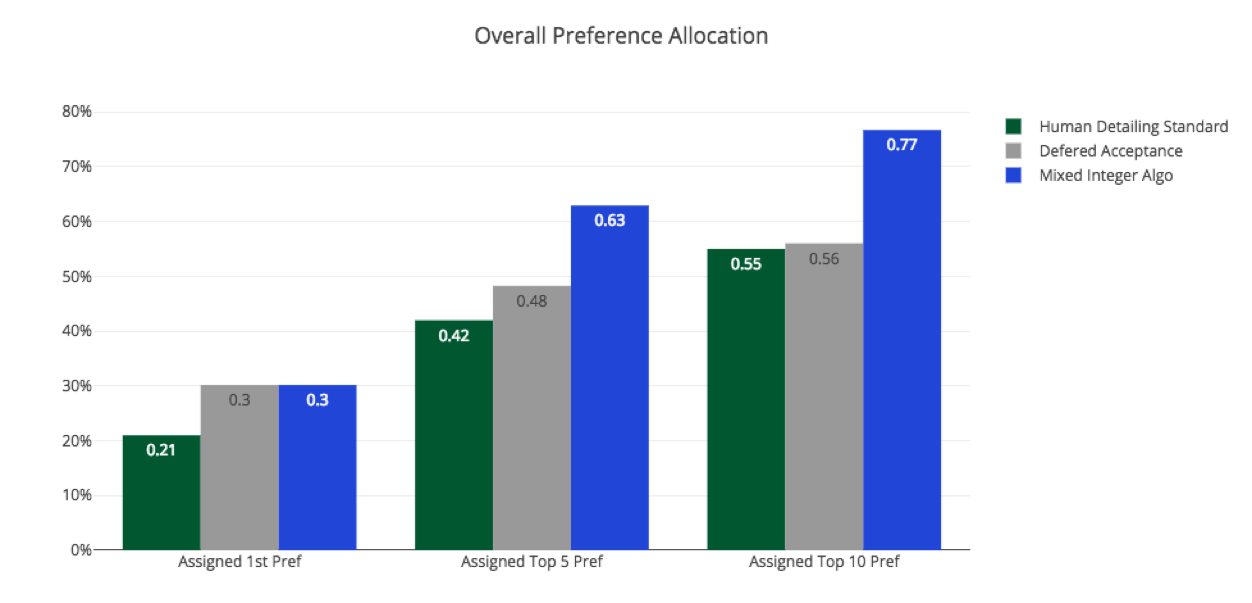
\includegraphics[scale=0.75]{Sections/figures/med_bar.png}
\end{center}

%As the below table shows, our algorithm performed better than deferred acceptance across squared average ranking. We chose squared average ranking as the comparative metric due to the view that in the markets we considered the desirability of a position decreases exponentially down ordinal rankings, not linearly.

%[Table]


\subsubsection{Post-Match Metrics Results}

The plot of Specialization vs. Competitiveness has a negative correlation. The negative correlation is expected and thus further validates the formulation.  A highly competitive market participant is desired by multiple firms, thus their skills generalize. A highly specialized market participant is desired strongly by few firms, making them un-competitive across the market when looked at in its entirety. Both competitive sailors and specialized sailors have a place in the Navy, and this metric validates their best placement. 

\begin{center}
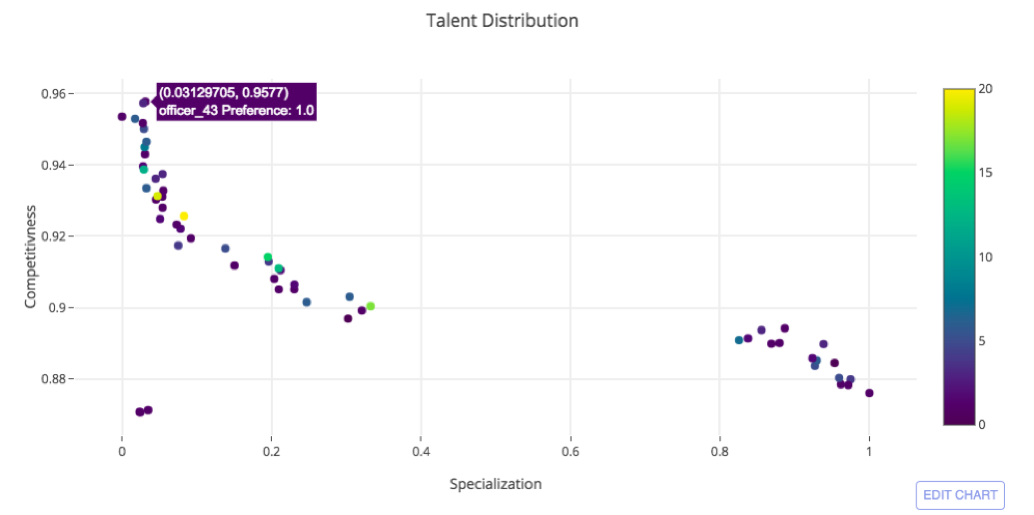
\includegraphics[scale=0.75]{Sections/figures/med_comp_v_spec.png}
\end{center}

%These plots for all our data sets can be found in Appendix (REF APPENDIX)

\section{Future Work}

\subsection{Inspired from Academia}

Ongoing work should continue to explore the best ways in which markets can be created. This includes consideration of partial matches or lotteries in MIP.\cite{1993_Roth} One may also consider the ability to explore the viability of leveraging Budish's wagering formulation of approximate competitive equilibrium from equal incomes.  \cite{2011_Budish} Additional research would include how to incorporate synergy of selection preferences by Job owners if allowed more than one person. \cite{1985_Roth_b}  Further, there could be that service members could be place in multiple jobs, such as selecting their main role and their collateral duties in the same matching process. \cite{1982_Roth} Lastly, an open question the authors are curious about is the opportunity for unsupervised learning (such as K-means clustering) on the preference data to see if there are clusters of service members with regards to their preferences, and what theres clusters indicate.

\subsection{Asks from DoD Personnel}

From interviewing DoD leadership there are several institution specific asks. Many of our considered markets have an “on-line” placement procedure \cite{1994_Khuller}, such as that which happens at many information-sensitive commands due to the trickle of clearance issuance as opposed to bulk assignment. 

In the same spirit of temporal considerations, military members have set time-lines at each command and are given expected rotation dates. Consideration of overlapping rotation and end strength could give another direction to objective function formulation.

Sometimes military members have the option to take orders or separate from the service. A future formulation could allow service members to express ordinal preference up to a point, and then indicate if they do not receive any of those they would opt to separate from the service. A constraint, we would imagine, would need to be added with respect to retention on each detailing cycle.

Tailored Compensation decisions could be made for uncompetitive, unspecialized positions the DoD needs filled.

Explore strategic importance of positions. This can either be an iteration where billets in priority tranche's are run iterative (tier 1 billets all matched, those sailors and billets are taken out of the pool, then tier 2 billets all matched, etc.), or a weighting where in a single matching optimization the preferences of higher tiered billets are given a greater weighting.

Forthcoming work on verifying and validating our implementation of inferred preferences will continually be bolstered as well \cite{2019_Shaw}.

\nocite{*}
\bibliography{Sections/DM}
\bibliographystyle{plain}

\newpage

\appendix
\appendixpage
\addappheadtotoc

\section{Notation}


Throughout the paper, we will reference the notation listed in this section.

\begin{align}
m &= \text{number of different jobs available}\\
n &= \text{number of persons}\\
\vec{P^S_i} &= \text{Preference vector of job seeker $i$, } \in \mathbb{Z}^{+, m \times 1} \\
P^S &= [\vec{P^S_i} | \dots | \vec{P^S_n}] \in \mathbb{Z}^{+, m \times n}, \\ 
&\text{\indent Preference Matrix of Seekers} \\
\vec{P^O_i} &= \text{Preference vector of job owner $j$, } \in \mathbb{Z}^{+, n \times 1} \\
P^O &= [\vec{P^O_i} | \dots | \vec{P^O_n}] \in \mathbb{Z}^{+, n \times m}, \\ 
&\text{\indent Preference Matrix of Job Owners} \\
\vec{A} &= \text{Position Available vector }\in \mathbb{Z}^{+, m \times 1} \\
a_j &= \text{Amount of positions for job $j$, } \in \mathbb{Z}^{+} \\
m_a &= \sum_i a_j \\
&= \text{ number of openings across Navy}\\
X &= \text{Placement Matrix} \in \{0,1\}^{n \times m} \\
x_{i,j} &= \begin{cases}
1 & \text{if $S_i$ is slated for job $j$}\\
0 & \text{otherwise}
\end{cases} \\
C &= \text{Co-Location Matrix, upper triangular}\\
C_{ij} &= \begin{cases}
1 & j > i, \text{ and  Seeker $i$ requests co-location with Seeker $j$} \\
0 & j\leq i, \text{ or Seeker $e_{i,1}$ does not request co-location}
\end{cases} \\
n_c &= \text{number of couples requesting co-location}\\
&= \frac{1}{2}\sum_{i=1}^n\sum_{j=1}^n C_{ij}\\
\end{align}



\newpage

\section{MIP Matching Formulation}
\label{Matching}

%Alternate to deterministic algorithms (such as Deferred Acceptance \cite{1962_Gale}) is a linear programming (optimization) approach. This allows system owners to input strategic objectives in the seeker-owner job matching process. The importance of job seeker preference can be weighted to be more important than owner, or vice versa. Requirements can also be added, as you will see in the formulation below.

The optimization function used in our investigation takes the form:

\begin{align}
\min \qquad & \sum_{i = 1}^{n} \sum_{j = 1}^{m} f(X_{ij}) \label{obj_func}\\
\text{ such that } \qquad & \sum_{j=1}^m X_{i,j} \leq 1 \quad  \forall i \in \{1, \dots n\} \label{one_job}\\
& \sum_{i = 1}^{i=n} \sum_{j = 1}^{m}X_{ij} = \min \left(n,\sum_{j = 1}^{m}a_j \right) \quad  \forall j \in \{1, \dots m\}  \label{all_filled}\\
& \sum_{i=1}^n X_{ij} \leq a_j \quad  \forall j \in \{1, \dots m\} \label{capacity} \\
& \sum \sum X_{ij}\mathbf{1}(X_{ij} P^S_{i} \leq w) \geq \sum \sum X_{ij}\mathbf{1}(X^{DA}_{ij} P^S_{i} \leq w) \quad \forall w \in \{1,5,10\} \\ \label{s_da}
& \sum \sum X_{ij}\mathbf{1}(X_{ij} P^O_{ji} \leq w) \geq \sum \sum X_{ij}\mathbf{1}(X^{DA}_{ij} P^O_{ji} \leq w) \quad \forall w \in \{1,5,10\} \\ \label{o_da}
\end{align}

The Goodness Function $f$ is the strategic objective function of the assignment process. For the sake of this paper, we set it to value the preference of the seeker twice as much as the preference of th job owner.

\[f(X_{ij}) = X_{ij}(P^S_{ij} + P^O_{ji})\]

\subsection{Matrix Formulation}

In matrix form this can be re-written (with $tr()$ indicating the trace):

\begin{align}
\min \qquad & tr(XP^O) + tr(X^TP^S) \label{mat_obj_func} \\
\text{ such that } \qquad & X^T \times 1^{m \times 1}  \leq 1  \label{one_job_matrix}\\
& (X \bullet 1)\bullet 1 = \min(n,A \bullet 1^{m \times 1}) \label{all_filled_matrix}\\
& X \times 1^{n \times 1} \leq A \label{capacity_matrix} \\
& \sum \sum X \bullet\mathbf{1}(X \bullet P^S \leq w) \geq \sum \sum X \bullet\mathbf{1}(X^{DA} \bullet P^S \leq w) \quad \forall w \in \{1,5,10\} \\ \label{mat_s_da}
& \sum \sum X \bullet\mathbf{1}(X \bullet (P^O)^T \leq w) \geq \sum \sum X \bullet\mathbf{1}(X^{DA} \bullet (P^O)^T \leq w) \quad \forall w \in \{1,5,10\} \\ \label{mat_o_da}
\end{align}

The proof for the equivalence of the objective functions (\ref{obj_func}) and (\ref{mat_obj_func}) is in Section \ref{mat_obj_func_proof}. The constraints in lines (\ref{one_job}) and (\ref{one_job_matrix}) ensure that each seeker receives only one job, lines (\ref{all_filled}) and (\ref{all_filled_matrix}) ensure that either all the jobs are filled or everyone has a job, lines (\ref{capacity}) and (\ref{capacity_matrix}) ensures that all jobs are at or below capacity (do not exceed capacity), and lines (\ref{s_da}, \ref{o_da}, \ref{mat_s_da}, \ref{mat_o_da}) ensure that our process is just as good or better in the post-match metrics of preference windows described in Section \ref{post-match}.

\subsubsection{Matrix formulation of Objective Function}
\label{mat_obj_func_proof}

\begin{align}
\sum_{i = 1}^{n} \sum_{j = 1}^{m} f(X_{ij}) &= \sum_{i = 1}^{n} \sum_{j = 1}^{m} X_{ji}\left(P^S_{ji} + P^O_{ij}\right)\\
&=   \sum_{j = 1}^{m}\sum_{i = 1}^{n} X_{ji}\left(\left(P^S\right)^T_{ij} + P^O_{ij}\right)\\
&=   \sum_{j = 1}^{m}\sum_{i = 1}^{n} X_{ji}\left(\left(P^S\right)^T + P^O\right)_{ij}\\
&=   \sum_{j = 1}^{m} \left( X\left(\left(P^S\right)^T + P^O \right)\right)_{jj}\\
&=   tr\left( X\left(\left(P^S\right)^T + P^O \right)\right)\\
%&= \sum_{i = 1}^{n} \sum_{j = 1}^{m} X_{ji}P^S_{ji} + \sum_{i = 1}^{n} \sum_{j = 1}^{m} X_{ji}P^O_{ij} \\
%&=  \sum_{i = 1}^{n} \sum_{j = 1}^{m} X^T_{ij}P^S_{ji} + \sum_{j = 1}^{m} \sum_{i = 1}^{n} X_{ji}P^O_{ij} \label{pre_jump}\\
%&= \sum_{i = 1}^{n} (X^TP^S)_{ii} + \sum_{j = 1}^{m}(XP^O)_{jj} \label{post_jump}\\
%&= tr(X^TP^S) + tr(XP^O)
\end{align}

\subsection{Formulation for CVXPY}

The difficulty with the constraints in lines (\ref{s_da}, \ref{o_da}, \ref{mat_s_da}, \ref{mat_o_da}) is that CVXPY does not have an indicator or filter atomic function that can be used in the objective function. Thus in order to code this formulation with the CWVPY we reformulated using the functions $\max$, which is an atomic function in the CVXPY API.

\begin{align}
x &= X_{ij} \\
p &= P^S_{ij} \\
g &\in \{1,5,10\} \\
\mathbf{1}(xp \leq g) &= \mathbf{1}(xp - g \leq 0) \\
&=  \mathbf{1}(\max(xp - g , 0) == 0) \\
&=  \max(1 - \max(xp - g , 0), 0) \\
\end{align}

The jump to the last line is made possible by the fact that $xp$ and $g$ are positive integers.


\newpage 

\section{MIP Co-Location Formulation}
\label{CoLocation}

The co-location constraint takes the form

\[ \frac{1}{n_c} \sum_{i=1}^{n}\sum_{j=i+1}^{n} \mathcal{D}(C_{ij}) \geq 0.95 \quad \texttt{at least 95\% of couples are co-located} \]

Distance Function $\mathcal{D}$ returns $1$ if the couple is considered co-located, 0 if not or if single. Here we choose 50 miles between job locations to be consider co-located because that is the threshold for receiving dislocation allowance (DLA) for a permanent change of station (PCS) according to the Joint Travel Regulations (JTR). The function $L(S_i)$ returns the location of the proposed station for Seeker $i$. 

\[\mathcal{D}(C_{ij}) = \begin{cases}
0 \quad & \text{ if } C_{ij}== 0 \\
 \mathbf{1}\big( || L(S_i) - L(S_j) || \leq 50 \big) \quad & \text{ otherwise }
 \end{cases}\]




\newpage

\section{MIP Quality Spread Formulation}
\label{QualitySpread}

There is precedent in the DoD to do assignments in a manner by which the distribution of quality officers is even accross some sort of grouping. This is the assignment policy for US Navy submariners to boats after initial training and US Marines to MArine Occupational Spectialties (MOS). The purpose of this is to ensure that no one unit or community within the force falls behind in competency due to a preponderance of low-performing personnel. 

To incorporate this into the matching algorithm would be easy. We would simply make the below formulation the objective function at (\ref{obj_func}).

\[ f(X) = \gamma \sum_{i=1}^n \sum_{j=1}^m X_{ij} \left(P^S_{ij} + P^O-{ji}\right) + \lambda (\sigma^2(X)) \]

The explanation of the objective function can be found below.

\begin{align*}
f(X) &= \gamma \sum_{i=1}^n \sum_{j=1}^m X_{ij} \left(P^S_{ij} + P^O-{ji}\right) + \lambda (\sigma^2(X)) \\
    \gamma, \lambda &= \texttt{weighting coefficient}, \in [0,1] \cap \mathbb{R} \\
    \sigma^2(X) &= \texttt{Variance of the quality assignments} \\
    \sigma^2(X) &= \frac{\sum_{j=1}^m (\mu^q_j - \bar{\mu^q})^2}{m-1} \\
    \mu^q_j &= \texttt{Average Quality score of person assigned to position } j \\
    \mu^q_j &= \sum_{i=1}^n  \frac{X_{ij} Q_i}{A_j} \\
    \bar{\mu^q} &= \sum_{j=1}^m \frac{\mu^q_j}{m} \\
    Q &= \texttt{Quality scores for each seeker }, \mathbb{R}^{n \times 1}
\end{align*}


\newpage

\section{MIP Importance Formulation}
\label{Importance}

Suppose service leadership were to favor some sort of command. This could look like giving operational commands twice the value preference over administrative commands, or favoring certain mission sets over others. This can easily be incorporated by a tweak to the objective function. 

\[f(X) = (P^S + WP^O)X \]

Here the vector $W \in \mathbb{R}^{m \times 1}$ is a weighting vector. For example, if the service leadership were to value a command \#1 which is highly operational twice that of any other command then

\[ W_i = \begin{cases} 2 & i = 1\\ 1 & \text{otherwise} \end{cases}\] 


\newpage

\section{MIP Retention Formulation}
\label{Retention}

Retention is often and important goal of military leaders wanting to maintain manpower numbers in order to keep the force ready for possible operations. The difficulty is, with an all volunteer force, if a service member is beyond contractual obligation, they need to have incentive to stay in. For example, a sailor may be willing to stay in for another 3 years if they are guaranteed to stay in San Diego so that their child can finish out high school there. If asked to move across the countryi, then they will opt to leave the service and seek local, civilian employment. 

For the purpose of maximizing retention (minimization is just a sign change), we can have the objective function (\ref{obj_func}) take the form below.

\begin{align*}
f(X) &= \gamma\left(\sum_{i=1}^n \sum_{j=1}^m X_{ij}(P^S_{ij} + P^O_{ji})\right) + \lambda (R(X)) \\
P^S_j &= \begin{cases}
m + 1 &  \text{Would rather separate than accept assignment to } j \\
[1,m] \cap \mathbb{Z}  &  \text{otherwise expressed preference} \\
\end{cases} \\ 
\gamma, \lambda &= \texttt{weighting coefficients}, \in [0,1] \cap \mathbb{R} \\
R(X) &= \texttt{Retention rate of assignment set }X \\
R(X) &= \frac{\sum_{i=1}^n \mathbf{1}\left(X\bullet P^S\right < m+1)}{n}
\end{align*}

We can also incorpoate retention as a constraint. Say a service leader were to desire retention above 90\%, then the following constraint would be necessary. 

\[R(X) \geq \texttt{Desired retention rate between 0 and 1} \]

Keep in mind, there is maximum rate on retention that is not necessarily 100\%, therefore when employing this constraint special care must be taken to guarantee feasibility.  

The maximum retention rate given the constraints of the college admission formulation (defined in lines (\ref{one_job}, \ref{all_filled}, \ref{capacity})), is the value of the objective function for the program described below. Keep in mind these constraints must be feasible for this analysis to be worthwhile; this requires that there is at least one solution where there are is at least one job seeker willing to fill each position in the market.

\begin{align*}
\max \qquad & R(X) \\
\text{ such that } \qquad & \sum_{j=1}^m X_{i,j} \leq 1 \quad  \forall i \in \{1, \dots n\} \\
& \sum_{i = 1}^{i=n} \sum_{j = 1}^{m}X_{ij} = \min \left(n,\sum_{j = 1}^{m}a_j \right) \quad  \forall j \in \{1, \dots m\}  \\
& \sum_{i=1}^n X_{ij} \leq a_j \quad  \forall j \in \{1, \dots m\}
\end{align*} 

We suspect the implementation of these retention in the objective function and/or constraints to be strategy proof (indicating it is in the best interest of market participants to honestly express their ordinal preferences) so long as the placements described in the output are enforced (as opposed to used for negotiation). Yet, we have not explored the strategy proofness rigorously and leave that investigation to future work.


\newpage

\section{More Results}

\subsection{Pre-Match Metrics}


\subsection{Post-Match Metrics}

\end{document}






